\documentclass[10pt,a4paper]{report}
\usepackage[latin1]{inputenc}
\usepackage{amsmath}
\usepackage{amsfonts}
\usepackage{amssymb}
\usepackage{graphicx}
\usepackage[danish]{babel}
\usepackage{hyperref}

\title{Webintelligence - Mini Project 1}
\author{Lars Andersen, Mathias Winde Pedersen \& S�ren Skibsted Als}
\begin{document}
	\maketitle
	
	\section*{Crawler}
	The crawler serves as the obtainer of website links. When doing this, it has to make sure that it follows the robots.txt specification.
	The robots.txt specification file, is a file that is placed at the root of websites, who wants to indicate what pages they want to have crawled by different search engines.
	This ensures explicit politeness.
	In order to not consume too much space, near duplicate detection is also performed here.
	The reason near duplicate detection is performed is that a large percentage of the internet content is duplicate information.
	
	We decided to implement the crawler with Mercator scheme.
	Mercator works by having several front and backqueues.
    The front queues serves as ranking of what websites gets crawled first.
    As an example, news sites can be put into a frontqueue with high priority, as such sites changes regularly, whereas a static site can have a lower priority for crawling.
    However, for the front queues we use a single queue, resulting in a uniform ranking, as we have no detection of what is static and what is dynamic websites.
    The backqueues makes you able to crawl different domains while still ensuring implicit politeness for the crawler.
    Implicit politeness being not hitting the same domain more than once every two seconds.
    
    
	Furthermore, the crawling is single threaded, as a proof of concept, but could be expanded to a multi threaded one.
	This is also related to DNS lookup times, as it was found that some DNS lookups delayed the crawler severely.
	
	An illustration of the Mercator scheme can be seen in Figure \ref{fig:mercator}
	\begin{figure}[h]
		\centering
		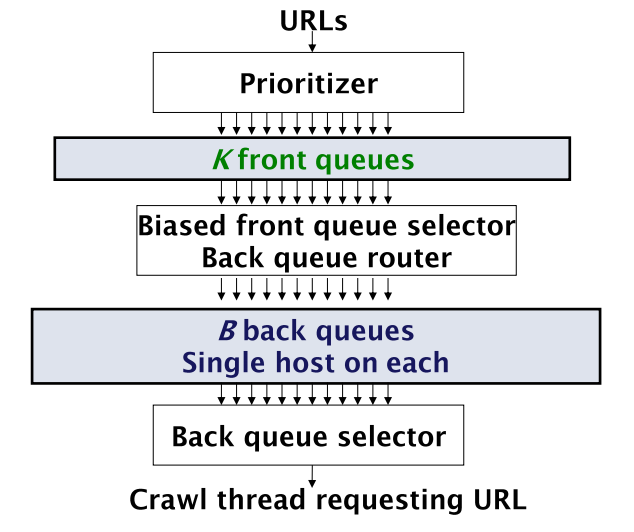
\includegraphics[scale=0.5]{mercator}
		\caption{Basic structure of Mercator Scheme, picture taken from slides.}\label{fig:mercator}
	\end{figure}
	
	
	To check near duplicates we use shingles with sketches.
	Shingles ia a continuous set of words, which in our case is a set of 8 words per shingle, thus a shingle size of 8, which is the size recommended by Google.
	Sketches is then to use hashing on these shingles, to reduce the storage necessary, as well as computation time, since the smallest of all the hashing values is chosen for each hash functions, and compares on this.
	However, Google recommends 84 hash functions for sketching, but we only use 19 hashes, as we did it as a proof of concept.
	
	Furthermore, tackling documents on the website which is not html or txt encoded is not handled, which gives crawled text encoded in a strange manner, e.g. pdf files.
	Image files are excluded, as some of those formats made the crawler otherwise crash, when trying to convert it to a string.
	A library could be used to translate such text into a readable format, to be used for the indexing, and also to make more sensible near duplicate detection.
	
	For the seed we used \url{http://aau.dk/} and \url{http://stackoverflow.com/}, which is the starting frontier of the crawler.
	A figure of the basic structure of a crawler can be seen in Figure \ref{fig:crawler}.
	\begin{figure}[h]
		\centering
		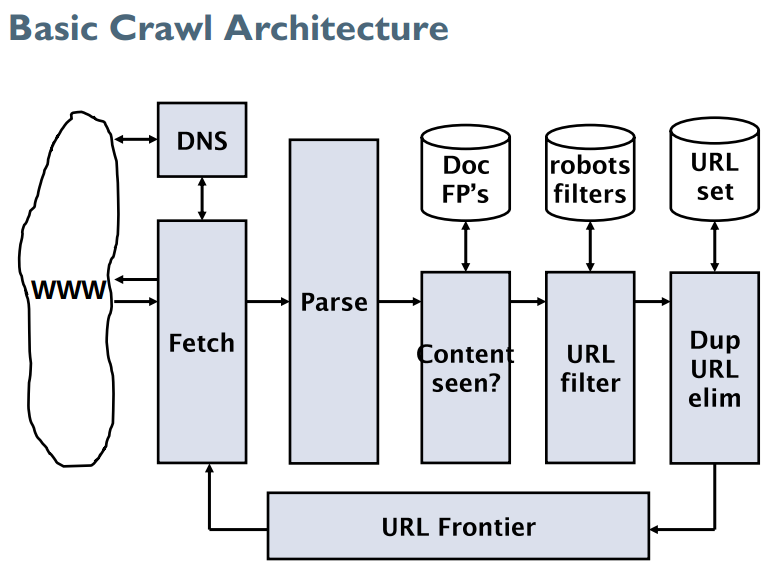
\includegraphics[scale=0.3]{basiccrawlarchitecture}
		\caption{Basic structure of crawler, picture taken from slides.}\label{fig:crawler}
	\end{figure}
	
	\section*{Indexer}
	The indexer has the purpose of constructing the inverted index, in that regard it is important to keep statistics of term and doc frequency, such that this information can be used by the ranker to rank pages.
	An inverted index is just similar to the back of a book, when you lookup a term, the pages containing the term are referenced.
	This provides the advantage that only documents containing the term are listed, and thus greatly reducing the memory required for storage.
	An example is a term only occuring on 100 out of 1 million sites crawled, then you only have to list 100 documents in the index, instead of the whole million, containing a lot of zeroes.
	
	For the indexer we cut corners as follows.
	We only stem on the English language.
	Stemming means cutting off unnecessary parts of the words to greatly reduce the index size.
	We do not develop our own stem method, but instead relies on an already developed one found on the web.
	
	For stopwords it is used for English and Danish,
	Which are common words without much meaning, such as "the", "about", "then", "by" etc.
	
	As we encode weird strings due to extracting pdf files without a library, we get some strange terms that fill the index unnecessarily.
	Services could be used to tackle such file formats, in order to extract the text from the pdf, word, and other such files.
	
	Furthermore, the postingslist are all kept in main memory. 
	This works fine for a small size of websites crawler, however, if you were to crawl the whole web, you would have to have servers farms or write to disk(making it much slower).
	
	A figure showing the basic steps of the indexer can be seen in Figure \ref{fig:indexer}. Where for the inverted index shown in the lower left, we also keep track of the amount of times the term occurs in the document, as that is used for the ranker.
	
	\begin{figure}[h]
		\centering
		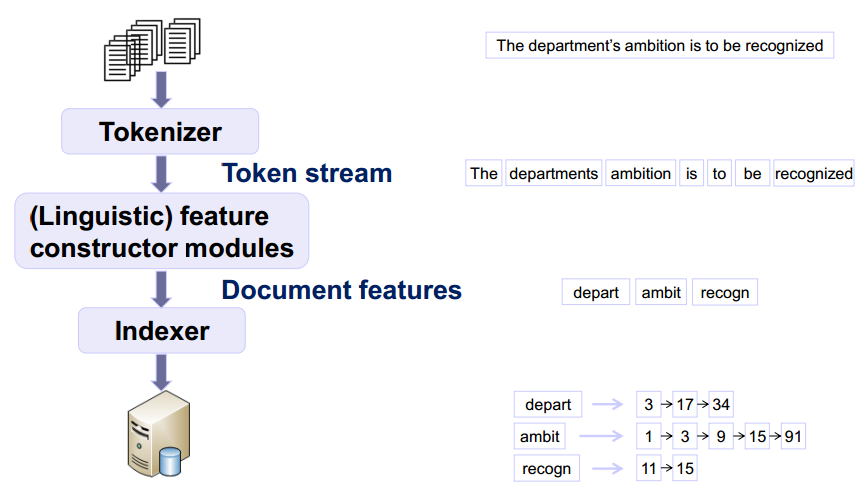
\includegraphics[scale=0.5]{indexer}
		\caption{Basic structure of Indexer, picture taken from slides.}\label{fig:indexer}
	\end{figure}
	
	\section*{Ranker}
	The ranker serves the purpose of ranking the pages, given a search query.
	
	 This is meaningful, as it contrary to boolean matching can weight different documents, and as of such can rank the results on what matches the query best, and not just if the terms occur in the document or not.
	
	For ranking we used the algorithm provided from the slideshow, which means we used the CosineScore, based on the tf-idf weighting.
	For contender pruning we used a precomputed champion list, which is a list of the $R$ documents for each term which has the highest weight.
	
	A picture of CosineScores can be seen in Figure \ref{fig:exampleconsinescore}.
	
	\begin{figure}[h]
		\centering
		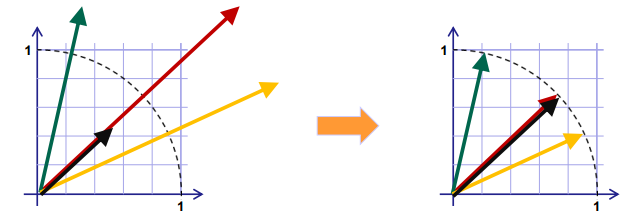
\includegraphics[scale=0.7]{CosineScore}
		\caption{Example of CosineScore, picture taken from slides.}
		\label{fig:exampleconsinescore}
	\end{figure}

	This made it possible to pre-compute this, and significantly reduce the computations needed when ranking, as the champion list limits each posting to a list of $r$ docs, the docs with the most occurrences of the given term the posting is associated with.
	
	A more specific description of the ranker comes here:
	The ranker takes a query as input and stems, uses stop-words and tokenizes, in the same manner as the indexer did for the documents, as the terms have to be treated in the same way, to locate them in the inverted index.
	
	The term frequency weight ($tf$) is the amount a given document contains the given term, where a logarithm is used as relevance is not proportional to frequency.
	$$log_{10} (1 + tf_{t,d})$$ 
	
	The document frequency is ($df$) is the total sum of occurrences of a term across all documents.
	the inverse document frequency ($id$f) can then be calculated as follows
	
	$$log_{10}(\frac{N}{df_t})$$
	Where N is the total amount of documents, which is 1000 in our case.
	
	The tf-idf weight, which is used for calculation of the score, can then be calculated as follows:
	$$tf-idf = tf*idf$$
	
	A small example, for calculating the score for a single document, given a query, can then be seen in Figure \ref{fig:exampleranking}
	\begin{figure}[h]
	\centering
	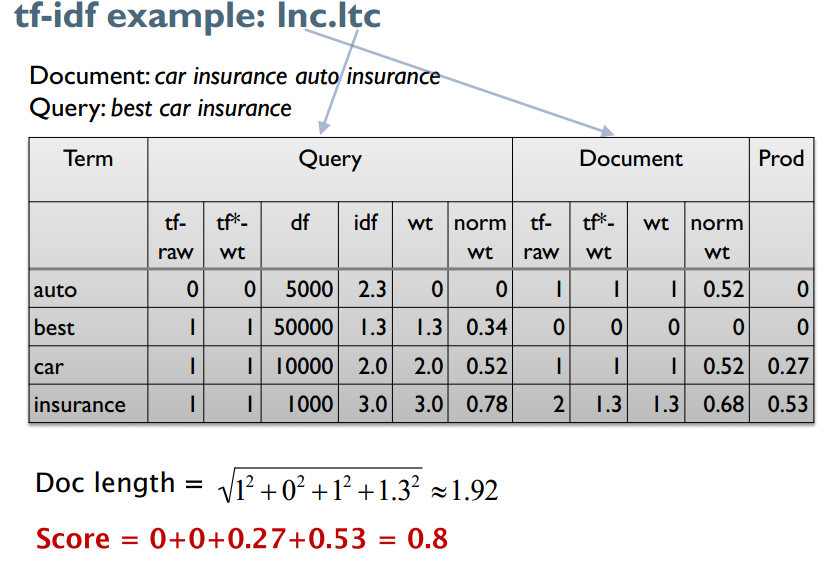
\includegraphics[scale=0.5]{exampleranking}
	\caption{Example of ranking score calculation, picture taken from slides.}\label{fig:exampleranking}
	\end{figure}
	
	Finally, to see how the crawler, indexer and ranker is structured in a broad sense, see Figure \ref{fig:bigpicture}
	
	\begin{figure}[h]
	\centering
	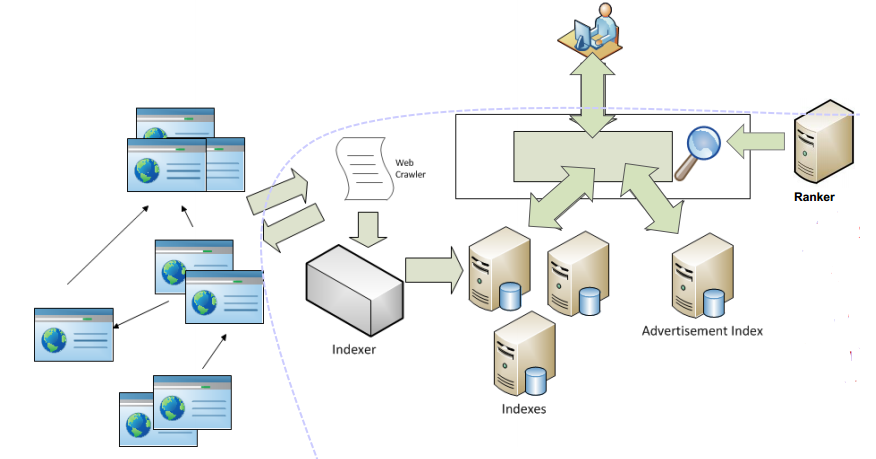
\includegraphics[scale=0.5]{generalarch}
	\caption{Basic structure of a search engine, picture taken from slides.}\label{fig:bigpicture}
	\end{figure}
	
	
\end{document}